\documentclass[a4paper, 14pt]{extarticle}
\usepackage[top=1in, bottom=1in, left=1in, right=1in]{geometry}
\usepackage{amsmath}
\usepackage{amssymb}
\usepackage{graphicx}
\usepackage{fontspec}
\usepackage{hyperref}
\usepackage{tikz}
\usepackage{fontspec}
%\usetikzlibrary{decorations.pathmorphing}
\usetikzlibrary{calc,decorations,patterns,arrows,decorations.pathmorphing,positioning}
\definecolor{pltblue}{HTML}{1F77B4}
\tikzset{every picture/.style={/utils/exec={\fontspec{Pretty Neat}}}}
\setmainfont{Pretty Neat}


\makeatletter
\pgfset{
  /pgf/decoration/randomness/.initial=2,
  /pgf/decoration/wavelength/.initial=100
}
\pgfdeclaredecoration{sketch}{init}{
  \state{init}[width=0pt,next state=draw,persistent precomputation={
    \pgfmathsetmacro\pgf@lib@dec@sketch@t0
  }]{}
  \state{draw}[width=\pgfdecorationsegmentlength,
  auto corner on length=\pgfdecorationsegmentlength,
  persistent precomputation={
    \pgfmathsetmacro\pgf@lib@dec@sketch@t{mod(\pgf@lib@dec@sketch@t+pow(\pgfkeysvalueof{/pgf/decoration/randomness},rand),\pgfkeysvalueof{/pgf/decoration/wavelength})}
  }]{
    \pgfmathparse{sin(2*\pgf@lib@dec@sketch@t*pi/\pgfkeysvalueof{/pgf/decoration/wavelength} r)}
    \pgfpathlineto{\pgfqpoint{\pgfdecorationsegmentlength}{\pgfmathresult\pgfdecorationsegmentamplitude}}
  }
  \state{final}{}
}
\tikzset{xkcd/.style={decorate,decoration={sketch,segment length=0.5pt,amplitude=0.5pt}}}
\makeatother

\usepackage{etoolbox}
\AtBeginEnvironment{tabular}{\fontspec{Pretty Neat}}

\setlength{\parindent}{0pt}
\setlength{\parskip}{0.5em}
\usepackage{fancyhdr}
\usepackage{geometry}
\usepackage{adjustbox}
\usepackage{titling}

\usepackage{amsmath}
\usepackage{amssymb}
\usepackage{graphicx}
\usepackage{hyperref}
\usepackage{tikz}
\usepackage{fontspec}
\usetikzlibrary{calc,decorations,patterns,arrows,decorations.pathmorphing}
\definecolor{pltblue}{HTML}{1F77B4}

\begin{document}

\section*{\fontspec{Pretty Neat}Who's the Big Cheese in the University Clubs?}
% Note: Replace 'XYZ123' with an actual image ID if you want to include a fun, relevant image

You're new at a university and want to understand social dynamics of students. Here's the club membership information:

\begin{center}
\begin{tabular}{|l|l|}
    \hline
    \textbf{Club} & \textbf{Members} \\
    \hline
    Drama Club & Sarah, Mike, Emma \\
    Art Club & Emma, Alex \\
    Volunteer Club & Alex, Olivia, James \\
    Sailing Club & Alex, Sophia \\
    Chess Club & Sophia, Ethan, Ava, Noah \\
    Debate Team & Noah, Lily \\
    Math Club & Noah, Lucas \\
    Tennis Club & Noah, Henry \\
    \hline
\end{tabular}
\end{center}

{\bf Question 1}:
Draw a network where students are nodes and edges connect students in the same club.

\clearpage

{\bf Question 2}:
Without doing any calculations, which student would you approach first if you wanted to spread information quickly about a new inter-club event? Explain your reasoning.

\vspace{8em}
{\bf Question 3}:
Without doing any calculations, which student would you recommend to be the "Club Coordinator" to help communication between different clubs? Explain your reasoning.

\vspace{8em}
{\bf Question 3}:
How might this network change if a new Robotics Club is formed, and Noan and Emma join it? How would this affect your answers to the previous questions?

\clearpage

{\bf Question 4}: Let's consider the following network:

\begin{center}
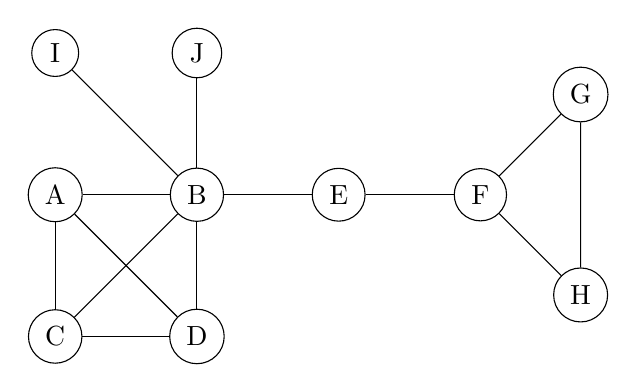
\begin{tikzpicture}[node distance=1.8cm]
    % Clique of four nodes
    \node[draw, circle] (A) {A};
    \node[draw, circle] (B) [right of=A] {B};
    \node[draw, circle] (C) [below of=A] {C};
    \node[draw, circle] (D) [right of=C] {D};
    \draw (A) -- (B) -- (D) -- (C) -- (A);
    \draw (A) -- (D);
    \draw (B) -- (C);

    % Intermediate node
    \node[draw, circle] (E) [right of=B] {E};
    \draw (B) -- (E);

    % Clique of three nodes
    \node[draw, circle] (F) [right of=E] {F};
    \node[draw, circle] (G) [above right of=F] {G};
    \node[draw, circle] (H) [below right of=F] {H};
    \draw (E) -- (F);
    \draw (F) -- (G) -- (H) -- (F);

    % Two nodes now attached to B
    \node[draw, circle] (I) [above of=A] {I};
    \node[draw, circle] (J) [right of=I] {J};
    \draw (B) -- (I);
    \draw (B) -- (J);
\end{tikzpicture}
\end{center}

Which node has the highest degree (most connections)?


{\bf Question 5}:

Nodes B, E, and F are likely the most central, being closest to all other nodes. Fill in the following table the distance from nodes B, E, and F to all nodes, and find the one with the shortest average distance.

\begin{center}
\begin{tabular}{|c|p{1cm}|p{1cm}|p{1cm}|p{1cm}|p{1cm}|p{1cm}|p{1cm}|p{1cm}|p{1cm}|p{1cm}|p{1cm}|}
\hline
& A & B & C & D & E & F & G & H & I & J & AVG \\
\hline
B & & & & & & & & & & & \\[0.5cm]
\hline
E & & & & & & & & & & & \\[0.5cm]
\hline
F & & & & & & & & & & & \\[0.5cm]
\hline
\end{tabular}
\end{center}

\clearpage

{\bf Question 6}:
Another way to think of centrality is based on how many shortest paths pass through a node.
For example, F appears in 14 shortest paths: from G and H (2 nodes) to A--E, I, and J (7 nodes).
Count the number of shortest paths that pass through nodes B and E. Which node is the most central by this measure?

\vspace{10em}

{\bf Question 7}: Going back to the school club network, which student would you approach first if you wanted to spread information quickly about a new inter-club event?

\vspace{3em}
{\bf Question 8}: Which student would you recommend to be the "Club Coordinator" to help communication between different clubs?

\vspace{3em}
{\bf Question 9}: How would the network change if a new Robotics Club is formed, and Noan and Emma join it? How would this affect your answers to the previous questions?

\end{document}